\documentclass[11pt,a4paper]{article}
			\usepackage[french]{babel}
					
				\usepackage{pifont}  
				\usepackage[utf8x]{inputenc}
				\usepackage[T1]{fontenc} 
				\usepackage{lmodern}			
				\usepackage{fancyhdr}
				\usepackage{textcomp}
				\usepackage{makeidx}
				\usepackage{tabularx}
				\usepackage{multicol}
				\usepackage{multirow}
				\usepackage{longtable}
				\usepackage{color}
				\usepackage{soul}
				\usepackage{boxedminipage}
				\usepackage{shadow}
				\usepackage{framed}			
				\usepackage{array}
				\usepackage{url}
				\usepackage{ragged2e}
				\usepackage{fancybox}
				\newcommand{\cadretitre}[2]{
				  \vspace*{0.8\baselineskip}
				  \begin{center}%
				  \boxput*(0,1){%
					%\colorbox{white}{\Large\textbf{\ #1\ }}%
				  }%
				  {%
					\setlength{\fboxsep}{10pt}%
				    \Ovalbox{\begin{minipage}{.8\linewidth}\begin{center}\Large\sffamily{#2}\end{center}\end{minipage}}}%
				  \end{center}
				  \vspace*{2\baselineskip}
				  }
			
			\makeatletter
			\def\@seccntformat#1{\protect\makebox[0pt][r]{\csname the#1\endcsname\quad}}
			\makeatother

				% Permet d'afficher qqchose à une positin absolue
				\usepackage[absolute]{textpos}
				\setlength{\TPHorizModule}{1cm}
				\setlength{\TPVertModule}{\TPHorizModule}
	
				\usepackage[titles]{tocloft}
				\setlength{\cftbeforesecskip}{0.5ex}
				\setlength{\cftbeforesubsecskip}{0.2ex}
				\addto\captionsfrench{\renewcommand\contentsname{}}
				
				\usepackage[font=scriptsize]{caption}
				
				\usepackage{listings}
\lstdefinestyle{lstverb}
  {
    basicstyle=\footnotesize,
    frameround=tttt, frame=trbl, framerule=0pt, rulecolor=\color{gray},
    lineskip=-1pt,   % pour rapprocher les lignes
    flexiblecolumns, escapechar=\\,
    tabsize=4, extendedchars=true
  }
\lstnewenvironment{Java}[1][]{\lstset{style=lstverb,language=java,#1}}{}
				\ifx\pdfoutput\undefined
					\usepackage{graphicx}
				\else
					\usepackage[pdftex]{graphicx}
				\fi
				\usepackage[a4paper, hyperfigures=true, colorlinks, linkcolor=black, citecolor=blue,urlcolor=blue, pagebackref=true, bookmarks=true, bookmarksopen=true,bookmarksnumbered=true,
                pdfauthor={}, pdftitle={TD Boucles}, pdfkeywords={TD Boucles, },pdfpagemode=UseOutlines,pdfpagetransition=Dissolve,nesting=true,
				backref, pdffitwindow=true, bookmarksnumbered=true]{hyperref}
				\usepackage{supertabular}
				\usepackage[table]{xcolor}
				\usepackage{url}
				\usepackage{caption} 
				\setlength{\parskip}{1.3ex plus 0.2ex minus 0.2ex}
				\setlength{\parindent}{0pt}
				
				\makeatletter
				\def\url@leostyle{ \@ifundefined{selectfont}{\def\UrlFont{\sf}}{\def\UrlFont{\footnotesize\ttfamily}}}
				\makeatother
				\urlstyle{leo}
				
				\definecolor{examplecolor}{rgb}{0.156,0.333,0.443}
				\definecolor{definitioncolor}{rgb}{0.709,0.784,0.454}
				\definecolor{exercisecolor}{rgb}{0.49,0.639,0}
				\definecolor{hintcolor}{rgb}{0.941,0.674,0.196}
				\definecolor{tableHeadercolor}{rgb}{0.709,0.784,0.454}
				\definecolor{tablerowAltcolor}{rgb}{.866,.905,.737}
				\definecolor{tablerowAlt2color}{rgb}{.968,.976,.933}
				\definecolor{verylightgray}{rgb}{0.98,0.98,0.98}
				
				\newenvironment{fshaded}{
				\def\FrameCommand{\fcolorbox{framecolor}{shadecolor}}
				\MakeFramed {\FrameRestore}}
				{\endMakeFramed}
				
				\newenvironment{fexample}[1][]{\definecolor{shadecolor}{rgb}{.913,.913,.913}
				\definecolor{framecolor}{rgb}{.156,.333,.443}
				\begin{fshaded}}{\end{fshaded}} 
				
				\newenvironment{fdefinition}{\definecolor{shadecolor}{rgb}{.913,.913,.913}
				\definecolor{framecolor}{rgb}{.709,.784,.454}
				\begin{fshaded}}{\end{fshaded}}
				
				\newenvironment{fexercise}{\definecolor{shadecolor}{rgb}{.913,.913,.913}
				\definecolor{framecolor}{rgb}{.49,.639,0}
				\begin{fshaded}}{\end{fshaded}}
				
				\newenvironment{fhint}{\definecolor{shadecolor}{rgb}{.913,.913,.913}
				\definecolor{framecolor}{rgb}{.941,.674,.196}
				\begin{fshaded}}{\end{fshaded}}	
				
				\newcommand{\PreserveBackslash}[1]{
				\let\temp=\\#1\let\\=\temp
				}
				\let\PBS=\PreserveBackslash
				\newcolumntype{A}{>{\PBS\raggedright\small\hspace{0pt}}X}
				\newcolumntype{L}[1]{>{\PBS\raggedright\small\hspace{0pt}}p{#1}}
				\newcolumntype{R}[1]{>{\PBS\raggedleft\small\hspace{0pt}}p{#1}}
				\newcolumntype{C}[1]{>{\PBS\centering\small\hspace{0pt}}p{#1}}
				
				\makeindex
				
				\title{TD Boucles}	
			\date{}
			\author{\scriptsize{}}
			\definecolor{light-gray}{gray}{0.8}
			\renewcommand{\headrulewidth}{0pt}
			\fancyhead[L]{
				\footnotesize\textsc{Haute \'Ecole de Bruxelles}\\
	    			\footnotesize\textsc{\'Ecole Sup\'erieure d'Informatique}
			}
			\fancyhead[R]{
				\footnotesize{Bachelor en Informatique}\\
				\footnotesize{Laboratoires Java} - 
			\footnotesize{1\`ere ann\'ee}}
				\fancyfoot[L]{ }
				\fancyfoot[C]{}
				\fancyfoot[R]{\scriptsize{\textcolor{gray}{version 2014-2015 (\today)}}}
				\pagestyle{plain}
				\reversemarginpar
				\usepackage{rotating}						
				\begin{document}
					\begin{textblock}{9}(2,3.2)
						
\includegraphics[width=2cm]{../../../_templates/java/icons/logo-esi}
					\end{textblock}
				
				
				
				
				%\maketitle
				\cadretitre{TD1}{TD Boucles}
				\thispagestyle{fancy}
        \marginpar{\begin{sideways}
            \begin{minipage}[t]{1cm}
            \begin{tiny}
            
\includegraphics[width=1\linewidth,height=1\textheight,keepaspectratio=true]{../../../_templates/java/icons/cc-gris.jpg}
			\end{tiny}
			\end{minipage}
            \begin{minipage}[b]{19cm}
            \begin{tiny}
            \textcolor{gray}{Distribué sous licence Creative Commons Paternité - Partage à l'Identique 2.0 Belgique 
            (\texttt{http://creativecommons.org/licenses/by-sa/2.0/be/})
			\vspace{-1em}
			\\Les autorisations au-delà du champ de cette licence peuvent être obtenues à 
			\texttt{http://www.heb.be/esi}
			- \texttt{mcodutti@heb.be}
			}\end{tiny}
			\end{minipage}
        \end{sideways}}
            \begin{abstract}
			Voyons ici comment incorporer des boucles, les structures r\'ep\'etitives, dans nos codes et comment les utiliser \`a bon escient.
    
            \par
        \end{abstract}
				\vspace{-2em}\tableofcontents
				\pagestyle{plain}
            \clearpage
            \fancyhead[L,C,R]{}
            \fancyfoot[L,C]{}
            \fancyfoot[R]{ \scriptsize{\textcolor{gray}{
				TDBoucle - page \thepage}}}
				\thispagestyle{fancy}
				\pagestyle{fancy}
	   
            \section{Les boucles}
        Si on veut faire effectuer un travail r\'ep\'etitif, il faut indiquer deux choses :
        
					\begin{enumerate}
				
			\item Le travail \`a r\'ep\'eter
			\item La mani\`ere de continuer la r\'ep\'etition ou de l'arr\^eter.
					\end{enumerate}
				
            \par
        \subsection{tant que}
        Le \guillemotleft  \verb@tant que@ \guillemotright  est une structure 
        qui demande \`a l'ex\'ecutant de r\'ep\'eter une t\^ache (une ou
        plusieurs instructions) tant qu'une condition donn\'ee est vraie.
      
            \par
        En pseudo-code :
            \par
        \begin{verbatim}
tant que condition faire
    séquence d’instructions à exécuter
fin tant que
      \end{verbatim}
        La \textbf{condition} est une expression d\'elivrant un r\'esultat 
        \textbf{bool\'een} (vrai ou faux).
      
            \par
        
        Il faut qu'il y ait dans la s\'equence d'instructions comprise entre \verb@tant que@
        et \verb@fin tant que@ au moins \textbf{une instruction qui 
        modifie} une des composantes de \textbf{la condition}
        de telle mani\`ere qu'elle puisse \textbf{devenir fausse} \`a un moment donn\'e. Dans le cas contraire,
        la condition reste \textbf{ind\'efiniment vraie} et la boucle va tourner sans fin, c'est ce qu'on appelle
        une \textbf{boucle infinie}.
      
            \par
        
        Si la condition est fausse d\`es le d\'ebut, la t\^ache n'est jamais ex\'ecut\'ee.
      
            \par
        \begin{figure}[hbt]
				    \begin{center}
					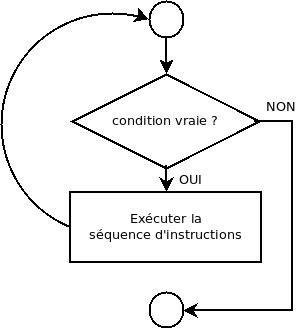
\includegraphics[width=0.8\linewidth,height=0.8\textheight,keepaspectratio=true]{/home/clr/Documents/Cours/DEV1Q2/TDBoucle/fr/image/boucleTq.jpg}
						\end{center}
                
                    \caption[boucleTq.jpg]{boucleTq.jpg}
                \end{figure}
                    
            \par
        Par exemple : 
            \par
        
			
		\subparagraph{Afficher les nombres plus petits que 10} 
		
					\textcolor{white}{.} \par
				On affiche uniquement les nombres inf\'erieurs (pas strictement) \`a 10 .
            \par
        \begin{verbatim}
// Affiche les nombres de 1 à 10.
algorithme compterJusque10 () // version avec tant que
    nb : entier
    nb ← 1 // c’est le premier nombre à afficher
    tant que nb ≤ 10 faire // c’est le premier nombre à afficher
      afficher nb  // on affiche la valeur de la variable nb
      nb ← nb + 1 // on passe au nombre suivant
    fin tant que
fin algorithme
      \end{verbatim}
			
		\subparagraph{Somme de nombres} 
		
					\textcolor{white}{.} \par
				 Apr\`es chaque nombre, on demande \`a l'utilisateur s'il y a encore un nombre \`a additionner.
            \par
        \begin{verbatim}
// Lit des valeurs entières et retourne la somme des valeurs lues.
algorithme sommeNombres() → entier
    valeur : entier // un des termes de l’addition
    somme : entier // la somme
    somme ← 0
    lire valeur
    tant que valeur ≥ 0 faire
      somme ← somme + valeur
      lire valeur // remarquer l’endroit où on lit une valeur.
    fin tant que
    retourner somme
fin algorithme
      \end{verbatim}\subsection{while}
		    L'\'equivalent Java de la boucle 
		  
            \par
        \begin{verbatim}
tant que condition faire
    séquence d’instructions à exécuter
fin tant que
      \end{verbatim}est 
            \par
        \begin{verbatim}
while ( condition ) {
    séquence d’instructions à exécuter
}
		  \end{verbatim}
			
		\subparagraph{Les puissances de 2} 
		
					\textcolor{white}{.} \par
				
            \par
        \begin{Java}
public class Util {

public static void puissance2() {
    int puissance = 1;
    while ( puissance < 100 ) {
      System.out. print(puissance + " ");
      puissance = 2 * puissance ;
    }
}\end{Java}affichera \verb@1 2 4 8 16 32 64 @
            \par
        
			
		\subparagraph{Somme d'entiers positifs} 
		
					\textcolor{white}{.} \par
				
            \par
        \begin{Java}
import java. util .Scanner;
public class Exemple {
    /**
     * Affiche la somme d entiers positifs entres au clavier .
     * S arrete des qu une valeur nulle ou negative est donnee.
     * @param args non utilise
    */
    public static void main(String [] args) {
      Scanner clavier = new Scanner(System.in);
      int nb;
      int somme = 0;
      nb = clavier . nextInt ();
      while ( nb > 0 ) {
        somme = somme + nb;
        nb = clavier . nextInt ();
      }
      System.out. println (somme);
    }
}\end{Java}affichera 0 si le premier nb lu vaut -5.
            \par
        
			
		\subparagraph{Un exemple complet} 
		
					\textcolor{white}{.} \par
				
            \par
        \begin{Java}
import java. util .Scanner;
public class Lecture {
    /**
    * Lit un entier au clavier .
    * Les valeurs non entieres sont passees .
    * @return l entier lu .
    */
    public static int lireEntier () {
      Scanner clavier = new Scanner(System.in);
      int nb;
      // Tant que ce n  est pas un entier au clavier
      while ( ! clavier .hasNextInt() ) {
        clavier .next (); // le lire , le passer
      }
      nb = clavier . nextInt ();
      return nb;
    }

    /**
    * Lit un entier au clavier .
    * Les valeurs non entieres , nulles ou negatives sont passees .
    * @return l entier lu .
    */
    public static int lirePositif () {
      int nb;
      nb = lireEntier ();
      while (nb<=0) {
        nb = lireEntier ();
      }
      return nb;
    }

    /**
    * Un exemple de main.
    */
    public static void main(String [] args){
      int nombreLu;
      
      System.out. print ("Entrez un entier  positif : ");
      nombreLu = lirePositif ();
    }
}\end{Java}\subsection{faire - tant que}\begin{verbatim}
faire
    séquence d’instructions à exécuter
tant que condition
      \end{verbatim}
        Cette structure est tr\`es proche du \guillemotleft  \verb@tant que@ \guillemotright  \`a une diff\'erence pr\`es :
        
					\begin{itemize}
				
			\item 
            Le \textbf{test} est fait \textbf{\`a la fin} et pas au d\'ebut. 
            La t\^ache est donc toujours \textbf{ex\'ecut\'ee au moins une fois}.
          
					\end{itemize}
				
            \par
        En pseudo-code :
            \par
        \begin{verbatim}
faire
    séquence d’instructions à exécuter
tant que condition
      \end{verbatim}
        La \textbf{condition} est une expression d\'elivrant un r\'esultat 
        \textbf{bool\'een} (vrai ou faux).
      
            \par
        
        Il faut que la s\'equence d'instructions comprise entre \verb@faire@ 
        et \verb@tant que@ contienne au moins 
        \textbf{une instruction qui modifie la condition} de telle mani\`ere 
        qu'elle puisse \textbf{devenir fausse} \`a un moment donn\'e pour arr\^eter l'it\'eration.
      
            \par
        
        La t\^ache est toujours \textbf{ex\'ecut\'ee au moins une fois}.
      
            \par
        \begin{figure}[hbt]
				    \begin{center}
					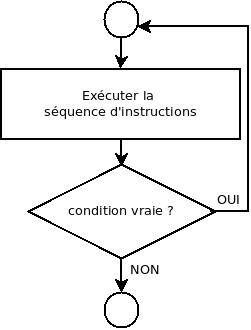
\includegraphics[width=0.8\linewidth,height=0.8\textheight,keepaspectratio=true]{/home/clr/Documents/Cours/DEV1Q2/TDBoucle/fr/image/boucleFaire.jpg}
						\end{center}
                
                    \caption[boucleFaire.jpg]{boucleFaire.jpg}
                \end{figure}
                    
            \par
        Par exemple : 
            \par
        
			
		\subparagraph{Somme de nombres} 
		
					\textcolor{white}{.} \par
				 Apr\`es chaque nombre, on demande \`a l'utilisateur s'il y a encore un nombre \`a additionner.
            \par
        \begin{verbatim}
// Lit des valeurs entières et retourne la somme des valeurs lues.
algorithme sommeNombres() → entier
    encore : booléen // est-ce qu’il reste encore une valeur à additionner ?
    valeur : entier // un des termes de l’addition
    somme : entier // la somme
    somme ← 0
    faire
      lire valeur
      somme ← somme + valeur
      lire encore
    tant que encore
    retourner somme
fin algorithme
      \end{verbatim}Avec cette solution, on additionne au moins une valeur.
            \par
        \subsection{do...while}
		    L'\'equivalent Java de la boucle 
		  
            \par
        \begin{verbatim}
faire
    séquence d’instructions à exécuter
tant que conditionPourResterDansLaBoucle
      \end{verbatim}est 
            \par
        \begin{verbatim}
do ( condition ) {
    séquence d’instructions à exécuter
} while( conditionPourResterDansLaBoucle );
		  \end{verbatim}
			
		\subparagraph{Les puissances de 2} 
		
					\textcolor{white}{.} \par
				
            \par
        \begin{Java}
public class Util {

public static void puissance2() {
    int puissance = 1;
    do {
      System.out. print(puissance + " ");
      puissance = 2 * puissance ;
    } while ( puissance < 100 );
}\end{Java}affichera \verb@1 2 4 8 16 32 64 @
            \par
        
			
		\subparagraph{Somme d'entiers positifs} 
		
					\textcolor{white}{.} \par
				
            \par
        \begin{Java}
import java. util .Scanner;
public class Exemple {
    /**
     * Affiche la somme d entiers positifs entres au clavier .
     * S arrete des qu une valeur nulle ou negative est donnee.
     * @param args non utilise
    */
    public static void main(String [] args) {
      Scanner clavier = new Scanner(System.in);
      int nb;
      int somme = 0;
      do{
        nb = clavier . nextInt ();
        somme = somme + nb;
      } while ( nb > 0 );
      System.out. println (somme);
    }
}\end{Java}affichera -5 si le premier nb lu vaut -5.
            \par
        \subsection{pour}
        On va indiquer combien de fois la t\^ache doit \^etre r\'ep\'et\'ee. Cela se fait au travers
        d'une \textbf{variable de contr\^ole} dont la valeur 
        va \'evoluer \textbf{\`a partir d'une valeur de d\'epart jusqu'\`a une valeur finale}.
      
            \par
        En pseudo-code :
            \par
        \begin{verbatim}
pour variable de début à fin [par pas] faire
    séquence d’instructions à exécuter
fin pour
      \end{verbatim} est \'equivalent \`a 
            \par
        \begin{verbatim}
{
variable : entier
variable ← début
tant que variable ≤ fin faire
    séquence d’instructions à exécuter
    variable ← variable + pas // ou variable ← variable + 1 si le pas est omis.
fin tant que
}
      \end{verbatim}
        Dans ce type de structure, \verb@début@, 
        \verb@fin@ et \verb@pas@ 
        peuvent \^etre des constantes, des variables ou
        des expressions (le plus souvent \`a valeurs enti\`eres mais on admettra parfois des r\'eels). 
      
            \par
        
        Le \verb@pas@ est facultatif, et g\'en\'eralement omis (dans ce cas, sa valeur par d\'efaut est 1). 
      
            \par
        
        Ce \verb@pas@ est parfois n\'egatif, dans le cas d'un compte \`a rebours, 
        par exemple \,\verb|pour n de 10 à 1 par -1|\,.
      
            \par
        
					\begin{enumerate}
				
			\item 
            Quand le \verb@pas@ est positif, 
            la boucle s'arr\^ete lorsque la \verb@variable@ 
            d\'epasse la valeur de \verb@fin@.
          
			\item 
            Par contre, avec un \verb@pas@ n\'egatif, 
            la boucle s'arr\^ete lorsque la \verb@variable@ 
            prend une valeur plus petite que la valeur de \verb@fin@.
          
					\end{enumerate}
				
            \par
        
        On consid\'erera qu'au cas (\`a \'eviter) o\`u
        
					\begin{enumerate}
				
			\item \verb@début@ est strictement sup\'erieur \`a \verb@fin@ 
            et le \verb@pas@ est positif, la s\'equence d'instructions n'est
            jamais ex\'ecut\'ee (mais ce n'est pas le cas dans tous les langages de programmation !). 
          
			\item 
            Idem si \verb@début@ est strictement inf\'erieur \`a \verb@fin@ 
            mais avec un \verb@pas@ n\'egatif.
          
					\end{enumerate}
				
            \par
        
        Attention de \textbf{ne pas modifier} dans la s\'equence d'instructions une des variables de contr\^ole
        \verb@début@, \verb@fin@ ou \verb@pas@ ! 
      
            \par
        
        Il est aussi fortement \textbf{d\'econseill\'e de modifier \guillemotleft  manuellement }\guillemotright  
        la \verb@variable@ 
        au sein de la boucle \verb@pour@. 
        Il ne faut pas l'initialiser en d\'ebut de boucle, et ne pas s'occuper de sa modification,
         l'instruction \verb@variable ← variable + pas@ \'etant automatique
        et implicite \`a chaque \'etape de la boucle. 
      
            \par
        
        Il est aussi d\'econseill\'e d'utiliser \verb@variable@ \`a la sortie
        de la structure \verb@pour@ sans lui affecter une nouvelle valeur.
      
            \par
        \begin{figure}[hbt]
				    \begin{center}
					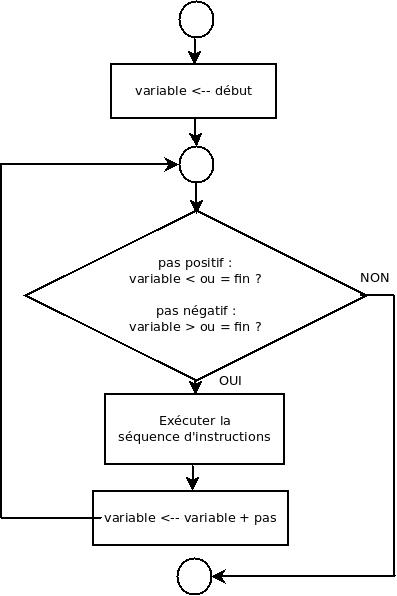
\includegraphics[width=0.8\linewidth,height=0.8\textheight,keepaspectratio=true]{/home/clr/Documents/Cours/DEV1Q2/TDBoucle/fr/image/bouclePour.jpg}
						\end{center}
                
                    \caption[bouclePour.jpg]{bouclePour.jpg}
                \end{figure}
                    
            \par
        Par exemple : 
            \par
        \begin{verbatim}
// Affiche les nombres de 1 à 10.
algorithme compterJusque10 () // version avec pour
    pour nb de 1 à 10 faire // par défaut le pas est de 1
      afficher nb
    fin pour
fin algorithme
    \end{verbatim}
			
		\subparagraph{Afficher les nombres plus petits que n} 
		
					\textcolor{white}{.} \par
				On affiche uniquement les nombres inf\'erieurs (pas strictement) \`a n.
            \par
        \begin{verbatim}
// Reçoit un nombre et affiche les nombres de 1 à ce nombre.
algorithme afficherN (n↓ : entier)
    pour nb de 1 à n faire
      afficher nb
    fin pour
fin algorithme
    \end{verbatim}
			
		\subparagraph{Afficher les nombres pairs plus petits que 10} 
		
					\textcolor{white}{.} \par
				On affiche uniquement les nombres pairs jusqu'\`a 10.
            \par
        \begin{verbatim}
// Reçoit un nombre et affiche les nombres pairs jusqu’à ce nombre.
// n : limite des nombres à afficher.
Exemple : si n vaut 10, les nombres pairs de 1 à 10 sont : 2, 4, 6, 8, 10.
algorithme afficherPair (n↓ : entier)
    pour nb de 2 à n par 2 faire
      afficher nb
    fin pour
fin algorithme
    \end{verbatim}
			
		\subparagraph{Afficher les nombres pairs plus petits que n} 
		
					\textcolor{white}{.} \par
				On affiche uniquement les nombres pairs jusqu'\`a la limite n.
            \par
        \begin{verbatim}
// Reçoit un nombre et affiche les nombres pairs jusqu’à ce nombre.
// n : limite des nombres à afficher.
// Exemple : si n vaut 10, les nombres pairs de 1 à 10 sont : 2, 4, 6, 8, 10.
algorithme afficherPair  (n↓ : entier)
    pour i de 1 à n DIV 2 faire
      afficher 2 * i
    fin pour
fin algorithme
    \end{verbatim}
			
		\subparagraph{Afficher n nombres pairs} 
		
					\textcolor{white}{.} \par
				On affiche les n premiers nombres pairs.
            \par
        \begin{verbatim}
// Reçoit un nombre et affiche ce nombre de nombres pairs.
// n: le nombre de nombres à afficher.
// Exemple : si n vaut 10, les 10 premiers nombres pairs sont : 2, 4, 6, 8, 10, 12, 14, 16, 18, 20.
algorithme afficherPair ()
    pour i de 1 à n faire
      afficher 2 * i
    fin pour
fin algorithme
    \end{verbatim}
			
		\subparagraph{Somme de nombres} 
		
					\textcolor{white}{.} \par
				L'utilisateur indique le nombre de termes au d\'epart.
            \par
        \begin{verbatim}
// Lit des valeurs entières et retourne la somme des valeurs lues.
algorithme sommeNombres () → entier
    nbValeurs : entier // nb de valeurs à additionner
    valeur : entier // un des termes de l’addition
    somme : entier // la somme
    somme ← 0 // la somme se construit petit à petit. Elle vaut 0 au départ
    demander nbValeurs
    pour i de 1 à nbValeurs faire
      lire valeur
      somme ← somme + valeur
    fin pour
    retourner somme
fin algorithme
    \end{verbatim}\subsection{for}
		    L'\'equivalent Java de la boucle 
		  
            \par
        \begin{verbatim}
pour variable de début à fin [par pas] faire
    séquence d’instructions à exécuter
fin pour
      \end{verbatim}est 
            \par
        \begin{verbatim}
for ( int i = début; i <= fin;  i = i+pas ) {
    séquence d’instructions à exécuter
}
  \end{verbatim}
			
		\subparagraph{Les nombres pairs entre 2 et 100} 
		
					\textcolor{white}{.} \par
				
            \par
        \begin{Java}
public class Exemple {
    /**
    * Affiche la somme des nombres pairs entre 2 et 100 inclus.
    * @param args non utilise
    */
    public static void main(String [] args) {
      int somme;
      somme = 0;
      for ( int i = 2; i <= 100; i = i+2 ) {
        somme = somme + i;
      }
      System.out. println (somme);
    }
}\end{Java}
			
		\subparagraph{Compte \`a rebours} 
		
					\textcolor{white}{.} \par
				
            \par
        \begin{verbatim}
public class Exemple {
    /**
    * Affiche un compte a rebours a partir de 10.
    * @param args non utilise
    */
    public static void main(String [] args) {
      for ( int i = 10; i >= 1; i = i−1 ) {
        System.out. println ( i );
      }
      System.out. println ("Partez !");
    }
}\end{verbatim}\verb@i++;@ est un raccourci pour \verb@i = i+1;@
            \par
        \begin{Java}
public class Exemple {
    /**
    * Affiche les nombres de 1 a 10 inclus.
    * @param args non utilise
    */
    public static void main(String [] args) {
      for ( int i = 1; i <= 10; i++ ) {
        System.out. println ( i );
      }
    }
}\end{Java}\subsection{Quel type de boucle choisir ?}
		    En pratique, il est possible d'utiliser syst\'ematiquement la boucle 
		    \verb@tant que@ qui peut s'adapter
        \`a toutes les situations. Cependant, 
        
					\begin{itemize}
				
			\item 
              il est plus clair d'utiliser la boucle \verb@pour@ 
              dans les cas o\`u le nombre d'it\'erations est fix\'e et connu \`a l'avance
              (par l\`a, on veut dire que le nombre d'it\'erations est d\'etermin\'e au moment o\`u on arrive \`a la boucle). 
            
			\item 
              La boucle \verb@faire@ convient quant \`a elle dans les cas o\`u le contenu de la boucle doit \^etre parcouru au moins une fois,
            
			\item 
              alors que dans \verb@tant que@, le nombre de parcours peut \^etre nul si la condition initiale est fausse.
            
					\end{itemize}
				
            \par
        \begin{figure}[hbt]
				    \begin{center}
					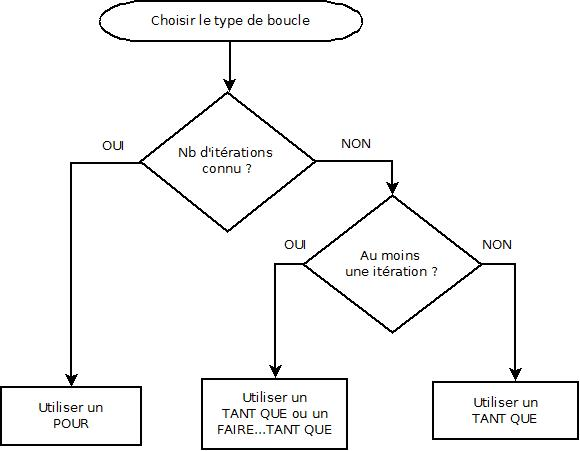
\includegraphics[width=0.8\linewidth,height=0.8\textheight,keepaspectratio=true]{/home/clr/Documents/Cours/DEV1Q2/TDBoucle/fr/image/boucleChoixType.jpg}
						\end{center}
                
                    \caption[boucleChoixType.jpg]{boucleChoixType.jpg}
                \end{figure}
                    
            \par
        \subsection{Sentinelle}
      Quand l'utilisateur entre une valeur sp\'eciale pour indiquer la fin 
      (d'une boucle \verb@tant que@ ou \verb@faire@), 
      on parle de\textbf{ valeur sentinelle}.
      Ceci n'est possible que si cette valeur sentinelle ne peut pas \^etre un terme valide. 
      Par exemple, si on veut additionner des nombres positifs uniquement, la valeur -1 peut
      servir de valeur sentinelle. Mais sans limite sur les nombres \`a additionner (positifs, n\'egatifs
      ou nuls) il n'est pas possible de choisir une sentinelle.
    \subsection{suite de nombres}
		    Un exemple simple pourrait \^etre celui-ci : 
		    \guillemotleft  \textit{\'Ecrire l'algorithme qui affiche les n premiers
        termes de la suite : 2, 4, 6. . . }\guillemotright 
      
            \par
        
        Puisqu'on doit \'ecrire plusieurs nombres et qu'on sait exactement combien, 
        on se tournera tout naturellement vers une boucle \verb@pour@.
      
            \par
        
        Le cas le plus simple est lorsque le nombre \`a afficher \`a l'\'etape \verb@i@ 
        peut \^etre calcul\'e en fonction de \verb@i@ seulement. L'algorithme est alors
      
            \par
        \begin{verbatim}
pour i de 1 à n faire
    afficher f(i)
fin pour
      \end{verbatim}Par exemple, pour afficher la suite des n premiers nombres pairs
            \par
        \begin{verbatim}
algorithme nombrePair (n↓ : entier)
    pour i de 1 à n faire
      afficher 2 * i
    fin pour
fin algorithme
      \end{verbatim}
        Parfois, il est difficile (voire impossible) de trouver \verb@f(i)@.\par
				
        On suivra alors une autre approche
        qui revient \`a calculer un nombre \`a afficher \`a partir du nombre pr\'ec\'edemment affich\'e (ou, plus
        exactement, de calculer le suivant \`a partir du nombre qu'on vient d'afficher). \par
				
        La structure g\'en\'erale est alors
      
            \par
        \begin{verbatim}
nb ← {1re valeur à afficher}
pour i de 1 à n faire
    afficher nb
    nb ← {calculer ici le nb suivant}
fin pour
      \end{verbatim}
        Dans l'exemple de la suite paire, le 1er nombre \`a afficher est 
        2 et le nombre suivant se calcule en ajoutant 2 au nombre courant.
      
            \par
        \begin{verbatim}
algorithme suite1 (n↓ : entier)
    nb : entier
    nb ← 2
    pour i de 1 à n faire
      afficher nb
      nb ← nb + 2
    fin pour
fin algorithme
      \end{verbatim}\subsection{3 pas en avant, 2 pas en arri\`ere}
		    Dans certains cas, il n'est pas possible de d\'eduire directement le nombre suivant en connaissant juste le nombre pr\'ec\'edent. 
		    Prenons un exemple un peu plus compliqu\'e pour l'illustrer.
		    \guillemotleft  \textit{\'Ecrire l'algorithme qui affiche les n premiers termes de la suite : 1, 2, 3, 4, 3, 2, 3, 4, 5, 4, 3. . }. \guillemotright 
      
            \par
        
        Si on vient d'\'ecrire, disons un 3, impossible sans information suppl\'ementaire, de connaitre
        le nombre suivant. Il faudrait savoir si on est en phase d'avancement ou de recul et combien
        de pas il reste \`a faire dans cette direction.
      
            \par
        
        Ajoutons des variables pour retenir l'\verb@état@ o\`u on est.
      
            \par
        \begin{verbatim}
algorithme suite3Avant2Arrière(n↓ : entier)
    nb, nbPasRestants, direction : entiers
    nb ← 1
    nbPasRestants ← 3 // 3 pas
    direction ← 1 // en avant
    pour i de 1 à n faire
      afficher nb
      nb ← nb + direction // faire un pas dans la bonne direction
      nbPasRestants ← nbPasRestants - 1
      si nbPasRestants = 0 alors // il est temps de changer de direction
        direction ← -direction
        si direction = 1 alors
          nbPasRestants ← 3
        sinon
          nbPasRestants ← 2
        fin si
      fin si
    fin pour
fin algorithme
      \end{verbatim}
        On obtient un algorithme plus long mais qui respecte toujours le sch\'ema vu.
      
            \par
        
        Un conseil : essayez de respecter ce sch\'ema et vous obtiendrez plus facilement un algorithme
        correct et lisible, \'egalement dans les cas particuliers.
      
            \par
        \section{La gestion des erreurs : try - catch}\subsection{L'instruction try catch}
					\begin{itemize}
				
			\item \verb@try@ : contient les instructions qui peuvent mal se passer
			\item \verb@catch@ : contient le code qui est en charge de g\'erer le probl\`eme
					\end{itemize}
				
        Quand un probl\`eme se pr\'esente dans le try
        
					\begin{itemize}
				
			\item Le code du \verb@try@ est interrompu
			\item Le code du \verb@catch@ est ex\'ecut\'e
			\item Ensuite, on continue apr\`es le \verb@try−catch@
					\end{itemize}
				
		  Exemple :
\begin{verbatim}
package be.heb.esi.lgj1 ;
import java.util.Scanner;
public class Affiche {
    /**
    * Affiche l ’ entier lu au clavier ou un message si ce n’ est pas un entier .
    * @param args inutilisé .
    */
    public static void main(String [] args) {
      Scanner clavier = new Scanner(System.in);
      int nb;
      try {
        nb = clavier . nextInt ();
        System.out. println (nb);
      }
      catch(Exception e) {
        System.out. println ("Ce␣n’est␣pas␣un␣entier!");
      }
    }
}
\end{verbatim}\section{Exercices}
				Maintenant, mettons tout \c ca en pratique.
      
            \par
        \subsection{Compr\'ehension d'algorithme}
          Pour ces exercices, nous vous demandons de comprendre des algorithmes donn\'es. 
          
			
		\subparagraph{Compr\'ehension} 
		
                \textcolor{white}{.} \par
            
							  Que vont-ils afficher ?
              
					\begin{itemize}
				
			\item \begin{verbatim}
algorithme boucle1 ()
    x : entier
    x ← 0
    tant que x < 12 faire
      x ← x+2
    fin tant que
    afficher x
finalgorithme
				\end{verbatim} \textcolor{gray}{\underline{\hspace*{2em}}} 
			\item \begin{verbatim}
algorithme boucle2 ()
    ok : booléen
    x : entier
    ok ← vrai
    x ← 5
    tant que ok faire
      x ← x+7
      ok ← x MOD 11 ≠ 0
    fin tant que
    afficher x
fin algorithme
				\end{verbatim} \textcolor{gray}{\underline{\hspace*{2em}}} 
			\item \begin{verbatim}
algorithme boucle3 ()
    ok : booléen
    cpt, x : entiers
    x ← 10
    cpt ← 0
    ok ← vrai
    tant que ok ET cpt < 3 faire
      si x MOD 2 = 0 alors
        x ← x+1
        ok ← x < 20
      sinon
        x ← x+3
        cpt ← cpt + 1
      fin si
    fin tant que
    afficher x
fin algorithme
				\end{verbatim} \textcolor{gray}{\underline{\hspace*{2em}}} 
			\item \begin{verbatim}
algorithme boucle4 ()
    pair, grand : booléens
    p, x : entiers
    x ← 1
    p ← 1
    faire
      p ← 2*p
      x ← x+p
      pair ← x MOD 2 = 0
      grand ← x > 15
    tant que NON pair ET NON grand
    afficher x
fin algorithme
				\end{verbatim} \textcolor{gray}{\underline{\hspace*{2em}}} 
			\item \begin{verbatim}
algorithme boucle5 ()
    i, x : entiers
    ok : booléen
    x ← 3
    ok ← vrai
    pour i de 1 à 5 faire
      x ← x+i
      ok ← ok ET (x MOD 2 = 0)
    fin pour
    si ok alors
      afficher x
    sinon
      afficher 2 * x
    fin si
fin algorithme
				\end{verbatim} \textcolor{gray}{\underline{\hspace*{2em}}} 
			\item \begin{verbatim}
algorithme boucle6 ()
    i, j, fin : entiers
    pour i de 1 à 3 faire
      fin ← 6 * i - 11
      pour j de 1 à fin par 3 faire
        afficher 10 * i + j
      fin pour
    fin pour
fin algorithme
				\end{verbatim} \textcolor{gray}{\underline{\hspace*{10em}}} 
					\end{itemize}
				
            \par
        \subsection{Compr\'ehension de codes Java}
			
		\subparagraph{Instructions r\'ep\'etitives} 
		
                \textcolor{white}{.} \par
            
							Quelles instructions r\'ep\'etitives sont correctes parmi les suivantes? 
							Expliquez pourquoi les autres ne le sont pas.
						
            \begin{itemize} 
        
            \item[ \ding{"6F} ] proposition 1
							\begin{Java}
While ( condition ) {
	// instructions
}							\end{Java}
        
            \item[ \ding{"6F} ] proposition 2
							\begin{Java}
do while ( condition ) {
	// instructions
}							\end{Java}
        
            \item[ \ding{"6F} ] proposition 3
							\begin{Java}
while ( true ) {
	// instructions
}							\end{Java}
        
            \item[ \ding{"6F} ] proposition 4
							\begin{Java}
while ( true ) do {
	// instructions
}							\end{Java}
        
            \item[ \ding{"6F} ] proposition 5
							\begin{Java}
FOR ( int i=0; i<=10; i=i+2 ) DO {
	// instructions
}							\end{Java}
        
            \item[ \ding{"6F} ] proposition 6
							\begin{Java}
for ( int i=0; i<=10; i=i+2 ) {
	// instructions
}							\end{Java}
        
            \item[ \ding{"6F} ] proposition 7
							\begin{Java}
for ( int i=0; i<=10; i=i+2 ) do {
	// instructions
}							\end{Java}
        
            \item[ \ding{"6F} ] proposition 8
							\begin{Java}
for ( int i=9; i>=0; i=i-2 ) {
	// instructions
}							\end{Java}
        
            \end{itemize} 
        
			
		\subparagraph{Activit\'e 'remplir les blancs'} 
		
                \textcolor{white}{.} \par
            
								Quel op\'erateur de comparaison Java repr\'esente la relation suivante? 
							
            \par
        
					\begin{enumerate}
				
			\item "est \'egal \`a" ?                      \textcolor{gray}{\underline{\hspace*{2em}}} 
			\item "est diff\'erent de" ?                \textcolor{gray}{\underline{\hspace*{2em}}} 
					\end{enumerate}
				
								Quel op\'erateur bool\'een Java repr\'esente l'op\'erateur logique suivant? 
							
            \par
        
					\begin{enumerate}
				
			\item le ET :   \textcolor{gray}{\underline{\hspace*{2em}}} 
			\item le OU :   \textcolor{gray}{\underline{\hspace*{2em}}} 
			\item le NON :  \textcolor{gray}{\underline{\hspace*{1em}}} 
					\end{enumerate}
				
			
		\subparagraph{Exp\'erience} 
		
					\textcolor{white}{.} \par
				
					Indiquez l'affichage obtenu par ce code.
				
            \par
        
			
		\subparagraph{} 
		
                \textcolor{white}{.} \par
            
							  Que vont-ils afficher ?
              \begin{Java}
public class Boucles {

	public static void main ( String[] args ) {
		int facteur;
		final int VALEUR = 3;
	
		for (facteur = 1 ; facteur <= 10 ; facteur++){		
			System.out.print(facteur*VALEUR+" ");
		}
		System.out.println();
	}
}			\end{Java} \textcolor{gray}{\underline{\hspace*{16em}}} 
			
		\subparagraph{Exercice Tant que} 
		
					\textcolor{white}{.} \par
				
					\'Ecrivez en Java l'algorithme suivant.
				
            \par
        \begin{verbatim}
algorithme Test

    nb, produit : Entier
    produit ← 1 

    demander nb
    tant que nb ≠ 0 faire
        produit ← produit * nb
        lire nb 
    fin tant que
    afficher produit
    
fin algorithme
			    \end{verbatim}
			
		\subparagraph{Exercice Pour} 
		
					\textcolor{white}{.} \par
				
					\'Ecrivez en Java l'algorithme suivant.
				
            \par
        \begin{verbatim}
algorithme Test

    nb: Entier
    i : Entier

    demander nb
    pour i de 1 à nb faire
        afficher i
    fin pour

fin algorithme
			     \end{verbatim}
			
		\subparagraph{Mots cl\'es} 
		
                \textcolor{white}{.} \par
            
							Compl\'etez le morceau de code suivant afin de pouvoir attraper l'exception de type \verb@IllegalArgumentException@ 
							susceptible d'\^etre lanc\'ee par la m\'ethode \verb@maxPositif@ de la m\^eme classe.
						\clearpage\begin{Java}
public static void appelMaxPositif() {

    Scanner clavier = new Scanner(System.in);
    
     \\_\\_\\_\\_  {
        int max = maxPositif(clavier.nextInt(), clavier.nextInt());
    }  \\_\\_\\_\\_\\_\\_\\_\\_  (IllegalArgumentException ex) {
        // gestion de l'exception
    }
    
}
							\end{Java}\subsection{\`A vous de jouer...}
          Voici quelques conseils pour vous guider dans la r\'esolution de tels probl\`emes :
          
					\begin{itemize}
				
			\item il convient d'abord de bien comprendre le probl\`eme pos\'e ; assurez-vous qu'il est parfaitement sp\'ecifi\'e ;
			\item r\'esolvez le probl\`eme via quelques exemples pr\'ecis ;
			\item mettez en \'evidence les variables \textbf{\guillemotleft  donn\'ees \guillemotright }, les variables \textbf{\guillemotleft  r\'esultats \guillemotright } et les variables de travail ;
			\item n'h\'esitez pas \`a faire une \'ebauche de r\'esolution en fran\c cais avant d'\'elaborer l'algorithme d\'efinitif pseudo-cod\'e ;
			\item d\'eclarez ensuite les variables (et leur type) qui interviennent dans chaque algorithme ; les noms des variables risquant de ne pas \^etre suffisamment explicites.
			\item \'Ecrivez la partie algorithmique \textbf{AVANT} de vous lancer dans la programmation en Java.
			\item Pour la partie Java, dessinez l'arborescence des fichiers, vous travaillerez dans un package  \verb@g12345.Boucles@. 
					\end{itemize}
				
            \par
        
        \'Ecrivez les algorithmes et codez les programmes Java correspondant qui 
          
					\begin{enumerate}
				
			\item re\c coit un naturel \verb@n@ et affiche
              
					\begin{enumerate}
				
			\item les \verb@n@ premiers entiers strictement positifs ;
			\item les \verb@n@ premiers entiers strictement positifs en ordre d\'ecroissant ;
			\item les \verb@n@ premiers carr\'es parfaits ;
			\item les \verb@n@ premiers naturels impairs ;
			\item les naturels impairs qui sont inf\'erieurs ou \'egaux \`a \verb@n@.
					\end{enumerate}
				
              Si le \verb@n@ re\c cu n'est pas strictement positif, votre programme g\'en\'erera une erreur/une exception 
              qui sera g\'er\'ee par un affichage explicite dans la m\'ethode \verb@main@.
            
			\item 
              demande \`a l'utilisateur d'introduire un entier positif (non strictement). 
              Cet algorithme permet \`a l'utilisateur de se tromper \`a plusieurs reprises mais l'utilisateur devra donner
              une bonne valeur pour arr\^eter le programme.
              (On suppose tout de m\^eme que l'utilisateur ne donne que des valeurs enti\`eres !) 
            
			\item 
              lit une s\'erie de nombres entiers positifs, jusqu'\`a ce que l'utilisateur
              encode la valeur 0. Les nombres multiples de 3 seront affich\'es au fur et \`a mesure et le nombre
              de ces multiples sera affich\'e en fin de traitement.
              
            \par
        
              Pensez \`a utiliser l'algorithme \'ecrit ci-dessus qui permet de lire un entier positif.
              
            \par
        
			\item 
              retourne la somme des chiffres qui forment un nombre naturel \verb@n@
              Attention, on donne au d\'epart le nombre et pas ses chiffres. Exemple : 133045 doit donner
              comme r\'esultat 16, car 1 + 3 + 3 + 0 + 4 + 5 = 16.
            
			\item 
              lit une suite de nombres positifs entr\'es au clavier et affiche
              le maximum, le minimum, leur somme et la moyenne. \par
				
              La fin de la suite de nombre sera signifi\'ee par une valeur sentinelle que vous choisirez
              judicieusement.
            
			\item 
              v\'erifie si un entier donn\'e forme un palindrome ou non. Un nombre
              palindrome est un nombre qui lu dans un sens (de gauche \`a droite) est identique au nombre
              lu dans l'autre sens (de droite \`a gauche). Par exemple, 1047401 est un nombre palindrome.
            
			\item 
                affiche les \verb@n@ premiers termes de la suite suivante : 
                \verb@1, –1, 2, –3, 5, –8, 13, –21, 34, –55, …@
                o\`u \verb@n@ est un entier strictement positif re\c cu en param\`etre.\par
				
                Si le \verb@n@ re\c cu n'est pas strictement positif, votre programme g\'en\'erera une erreur/une exception 
                qui sera g\'er\'ee par un affichage explicite dans la m\'ethode \verb@main@.
            
					\end{enumerate}
				
            \par
        En java, n'oubliez pas d'\'ecrire la javadoc et la m\'ethode main pour tester vos m\'ethodes.
            \par
        
			
		\subparagraph{Jeu de la fourchette} 
		
					\textcolor{white}{.} \par
				
          \'Ecrivez un algorithme qui simule le jeu de la fourchette. Ce jeu consiste \`a essayer de d\'ecouvrir
          un nombre quelconque compris entre 0 et 100 inclus, tir\'e au sort par l'ordinateur (la primitive
          \verb@hasard(n : entier)@ retourne un entier entre 1 inclus et n exclus). \par
				
          L'utilisateur a droit \`a huit essais maximum.\par
				
          \`A chaque essai, l'algorithme devra afficher un message indicatif
          
					\begin{itemize}
				
			\item \guillemotleft  nombre donn\'e trop petit \guillemotright 
			\item ou \guillemotleft  nombre donn\'e trop grand \guillemotright . 
					\end{itemize}
				
          En conclusion, 
          
					\begin{itemize}
				
			\item soit \guillemotleft  bravo, vous avez trouv\'e en [nombre] essai(s) \guillemotright 
			\item soit \guillemotleft  d\'esol\'e, le nombre \'etait [valeur] \guillemotright .
					\end{itemize}
				
            \par
        \'Ecrivez le code java correspondant.
            \par
        
        Aide en Java : un petit tour dans l'API de la classe Random devrait vous aider \`a trouver l'\'equivalent du
        \verb@hasard(n : entier)@ en Java
    
            \par
        
				\end{document}
			